\section{Results}
\label{section:results}

\subsection{Genetic algorithm}
In figures 3 and 4 are shown the results of the evolution of the configuration vector \(c\in\mathcal{C}\) by means of the genetic algorithom described in \textit{Method}. The best individual after ca. 30 generations was tested against best programmer-defined configuration in a 1 vs. 1 scenario where they were instructed to move the ball into the other player's goal. If none of the players had managed to score a goal after 60 seconds, the game was counted as a draw. The results of 25 games is shown in figure 5.

\begin{figure}[tbp]
\centering
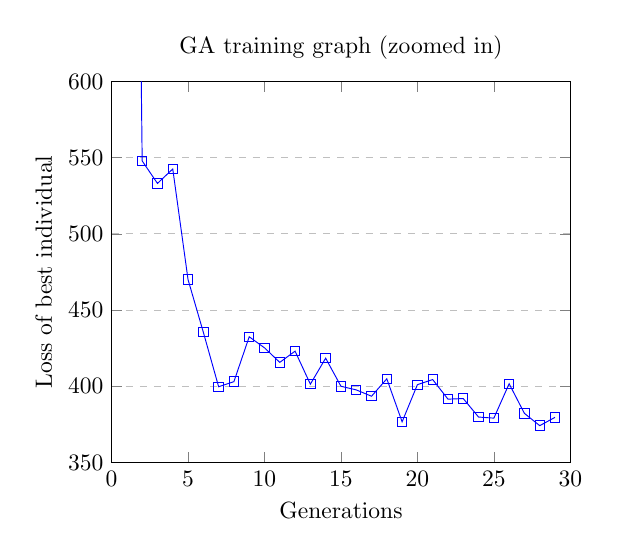
\begin{tikzpicture}[scale=0.85]
\begin{axis}[
    title={GA training graph (zoomed in)},
    xlabel={Generations},
    ylabel={Loss of best individual},
    xmin=0, xmax=30,
    ymin=350, ymax=600,
    xtick={0,5,10,15,20,25,30},
    ytick={300,350,400,450,500,550,600,650,700,750,800,850,900,950,
    1000,1050,1100,1150,1200,1250,1300,1350,1400,1450,1500},
    %ytick={300,400,500,600,700,800,900,1000,1100,1200,1300,1400,1500},
    legend pos=north west,
    ymajorgrids=true,
    grid style=dashed,
]

\addplot[
    color=blue,
    mark=square,
    ]
    coordinates {
(1,1436.1875)(2,547.875)(3,533.125)(4,542.59375)(5,470.0)(6,435.5)(7,399.71875)(8,403.0625)(9,432.5)(10,425.25)(11,415.71875)(12,423.0625)(13,401.40625)(14,418.46875)(15,400.03125)(16,397.65625)(17,393.5)(18,404.9375)(19,376.71875)(20,401.0625)(21,404.4375)(22,391.59375)(23,391.96875)(24,379.84375)(25,379.125)(26,401.6875)(27,382.25)(28,374.1875)(29,379.65625)
    };


\end{axis}
\end{tikzpicture}
	\caption{Graph showing the loss function of the best individual through generations.}
\end{figure}



\begin{figure}[h]
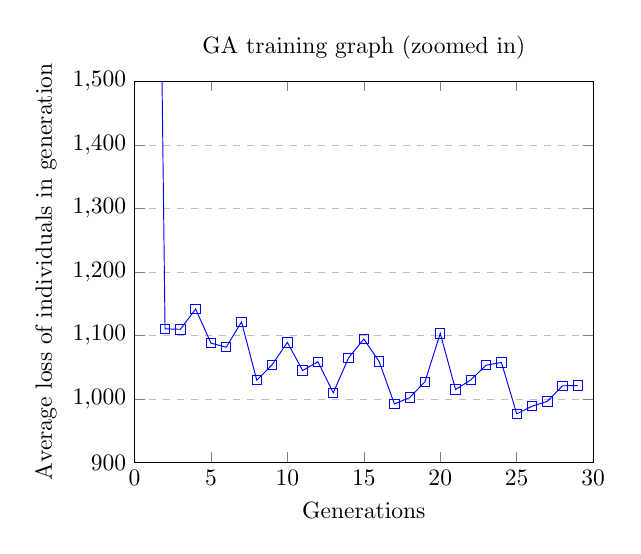
\begin{tikzpicture}[scale=0.85]
\begin{axis}[
    title={GA training graph (zoomed in)},
    xlabel={Generations},
    ylabel={Average loss of individuals in generation},
    xmin=0, xmax=30,
    ymin=900, ymax=1500,
    xtick={0,5,10,15,20,25,30},
    %ytick={300,350,400,450,500,550,600,650,700,750,800,850,900,950,
    %1000,1050,1100,1150,1200,1250,1300,1350,1400,1450,1500},
    %ytick={500,1000,1500,2000,2500,3000,3500},
    ytick={900,1000,1100,1200,1300,1400,1500},
    legend pos=north west,
    ymajorgrids=true,
    grid style=dashed,
]

\addplot[
    color=blue,
    mark=square,
    ]
    coordinates {
(1,3098.46875)(2,1110.4375)(3,1109.7916666666667)(4,1141.7135416666667)(5,1087.9895833333333)(6,1081.5625)(7,1121.390625)(8,1029.5989583333333)(9,1053.84375)(10,1089.21875)(11,1044.875)(12,1058.734375)(13,1009.7395833333334)(14,1064.5989583333333)(15,1094.4947916666667)(16,1059.1302083333333)(17,992.2916666666666)(18,1002.25)(19,1027.1927083333333)(20,1103.2864583333333)(21,1014.921875)(22,1030.1770833333333)(23,1053.2135416666667)(24,1057.5364583333333)(25,976.6666666666666)(26,988.5833333333334)(27,996.3333333333334)(28,1020.8177083333334)(29,1021.2708333333334)
    };


\end{axis}
\end{tikzpicture}
	\caption{Graph showing the mean value of the loss function for each individual through generations.}
\end{figure}

\begin{figure}[h]
\begin{tabular}{lllll}
\cline{1-3}
\multicolumn{1}{|l|}{GA wins}         & \multicolumn{1}{l|}{18} & \multicolumn{1}{l|}{72\%} &  &  \\ \cline{1-3}
\multicolumn{1}{|l|}{Programmer wins} & \multicolumn{1}{l|}{4}  & \multicolumn{1}{l|}{16\%} &  &  \\ \cline{1-3}
\multicolumn{1}{|l|}{Draws}           & \multicolumn{1}{l|}{3}  & \multicolumn{1}{l|}{12\%} &  &  \\ \cline{1-3}
\end{tabular}
		\caption{Results of GA-vs-programmer experiment shown in amount and percentage.}
\end{figure}

\subsection{rcssserver}
The use of rcssserver led to achieving a basic but working simulation that was used to perform the training for the genetic algorithm.

\subsection{Reinforcement Learning}
The experiments with reinforcement learning did not give the desired results.  
Even in basic scenarios, the agent was not able to score goals consistently.  
Training in a basic two-player setup did not show any coordinated and cooperative play between the two players.  
The players run towards the ball slowly and dribble towards the goal.  
Shooting was hard to replicate even in simplified scenarios.  

\subsection{Rule-Based System}
The best results were achieved when the blue agents utilized a Rule-Based System. When employing the Rule-Based System, 
the blue team consistently outperformed the hardcoded red team, winning every simulated match.
